% answers.tex —— 2008 年·普通高等学校招生考试·福建卷·理科 · 参考答案与详细解析片段
% 由 tools/generate_projects.py 依来源总账自 2008/2008_数学真题_福建理_试题.md + 2008/2008_数学真题_福建理_解析正文.md + 2008/2008_数学真题_福建理_答案要点.md 生成，勿手改（改源 MD 后重跑）


\begin{gktip}
固定候选 PDF 仅含题面，无答案、解析和评分标准，原卷亦未标注分值；以下为非官方编者独立推导，官方答案字段为空。来源发布者、出版者、版次与官方身份均未核。
\end{gktip}

\begin{answer}
\gksolhead{1}{}

\textbf{题目}：

若复数 $(a^2-3a+2)+(a-1)\mathrm i$ 是纯虚数，则实数 $a$ 的值为（　）

（A）$1$

（B）$2$

（C）$1$ 或 $2$

（D）$-1$

\Needspace{4\baselineskip}
\textbf{解析}

\Needspace{5\baselineskip}
纯虚数要求实部为零而虚部不为零：

\nopagebreak[4]
\[a^2-3a+2=0\iff a=1\text{ \text{或} }2.\]

当 $a=1$ 时虚部 $a-1=0$，不合；故 $a=2$。

\gkanswer{答案：B。}

\end{answer}
\begin{answer}
\gksolhead{2}{}

\textbf{题目}：

设集合 $A=\left\{x\mid \dfrac{x}{x-1}<0\right\}$，$B=\{x\mid 0<x<3\}$，那么“$m\in A$”是“$m\in B$”的（　）

（A）充分而不必要条件

（B）必要而不充分条件

（C）充要条件

（D）既不充分也不必要条件

\Needspace{4\baselineskip}
\textbf{解析}

由 $\dfrac{x}{x-1}<0$ 得 $0<x<1$，即 $A=(0,1)$，而 $B=(0,3)$，故 $A\subsetneq B$，“$m\in A$”是“$m\in B$”的充分不必要条件。

\gkanswer{答案：A。}

\end{answer}
\begin{answer}
\gksolhead{3}{}

\textbf{题目}：

设 $\{a_n\}$ 是公比为正数的等比数列，若 $a_1=7$，$a_5=16$，则数列 $\{a_n\}$ 前 $7$ 项的和为（　）

（A）$63$

（B）$64$

（C）$127$

（D）$128$

\Needspace{4\baselineskip}
\textbf{解析}

\Needspace{5\baselineskip}
【源疑点：原页印作 $a_1=7$，$a_5=16$。按此 $q^4=\dfrac{16}7$，$S_7=7\cdot\dfrac{q^7-1}{q-1}\approx98.8$，不在四个选项内。若按与选项自洽的 $a_1=1$（$q^4=16$，$q=2$），则

\nopagebreak[4]
\[S_7=1+2+\cdots+64=127,\]

对应选项 (C)。本库题面照原页转录，作答从选项口径。】

\gkanswer{答案：C。}

\end{answer}
\begin{answer}
\gksolhead{4}{}

\textbf{题目}：

函数 $f(x)=x^3+\sin x+1$（$x\in\mathbf R$），若 $f(a)=2$，则 $f(-a)$ 的值为（　）

（A）$3$

（B）$0$

（C）$-1$

（D）$-2$

\Needspace{4\baselineskip}
\textbf{解析}

\Needspace{5\baselineskip}
由 $f(a)=a^3+\sin a+1=2$ 得 $a^3+\sin a=1$，于是

\nopagebreak[4]
\[f(-a)=-a^3-\sin a+1=-1+1=0.\]

\gkanswer{答案：B。}

\end{answer}
\begin{answer}
\gksolhead{5}{}

\textbf{题目}：

某一批花生种子，如果每 $1$ 粒发芽的概率为 $\dfrac45$，那么播下 $4$ 粒种子恰有 $2$ 粒发芽的概率是（　）

（A）$\frac{16}{625}$

（B）$\frac{96}{625}$

（C）$\frac{192}{625}$

（D）$\frac{256}{625}$

\Needspace{4\baselineskip}
\textbf{解析}

\Needspace{5\baselineskip}
四次独立试验中恰有两次发芽：

\nopagebreak[4]
\[P=\mathrm C_4^2\left(\frac45\right)^2\left(\frac15\right)^2=6\times\frac{16}{25}\times\frac1{25}=\frac{96}{625}.\]

\gkanswer{答案：B。}

\end{answer}
\begin{answer}
\gksolhead{6}{}

\textbf{题目}：

如图，在长方体 $ABCD-A_1B_1C_1D_1$ 中，$AB=BC=2$，$AA_1=1$，则 $BC_1$ 与平面 $BB_1D_1D$ 所成角的正弦值为（　）

（A）$\frac{\sqrt6}{3}$

（B）$\frac{2\sqrt6}{5}$

（C）$\frac{\sqrt{15}}{5}$

（D）$\frac{\sqrt{10}}{5}$
\nopagebreak[4]
\begin{center}% 2008 年福建卷理科第 6 题：长方体 ABCD-A1B1C1D1，AB=BC=2，AA1=1，
%   求 BC1 与平面 BB1D1D 所成角的正弦值。
% 来源 PDF：gaokaomath-src/普通高考/2008/2008福建理.pdf
% SHA-256：516e8ac8e113868afa9bc4af4724c3b43f22a1f7fecc830a7f3400b8d973d452
% 原页：2008福建理.pdf 第 1 页（A3 三栏）第 1 栏，书页码 441。
% 重绘依据：按原页斜投影：A 前左下、B 前右下、C 右侧、D 被遮挡；A1、B1、C1、D1 为对应顶点；
%   A—D、D—C、D—D1、B—D 虚线，其余棱与对角线 BC1 实线。
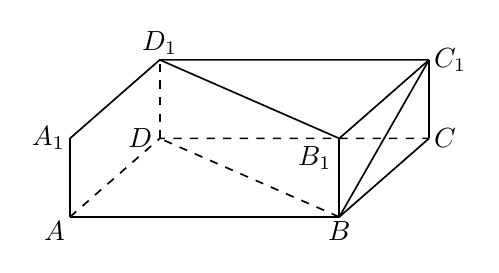
\begin{tikzpicture}[scale=0.95, semithick, every node/.style={inner sep=1.5pt}]
  \coordinate (A) at (0.00,0.00);
  \coordinate (B) at (3.60,0.00);
  \coordinate (C) at (4.80,1.05);
  \coordinate (D) at (1.20,1.05);
  \coordinate (A1) at (0.00,1.05);
  \coordinate (B1) at (3.60,1.05);
  \coordinate (C1) at (4.80,2.10);
  \coordinate (D1) at (1.20,2.10);

  \draw (A) -- (B) -- (C);
  \draw (A) -- (A1);
  \draw (B) -- (B1);
  \draw (C) -- (C1);
  \draw (A1) -- (D1) -- (C1);
  \draw (D1) -- (B1);
  \draw (B1) -- (C1);
  \draw (B) -- (C1);

  \draw[dashed] (A) -- (D) -- (C);
  \draw[dashed] (D) -- (D1);
  \draw[dashed] (B) -- (D);

  \node[below left] at (A) {$A$};
  \node[below] at (B) {$B$};
  \node[right] at (C) {$C$};
  \node[left=1pt] at (D) {$D$};
  \node[left] at (A1) {$A_1$};
  \node[below left=1pt] at (B1) {$B_1$};
  \node[right] at (C1) {$C_1$};
  \node[above] at (D1) {$D_1$};
\end{tikzpicture}
\end{center}
\nopagebreak[4]
\Needspace{4\baselineskip}
\textbf{解析}

\Needspace{5\baselineskip}
以 $A$ 为原点，$AB$、$AD$、$AA_1$ 为 $x$、$y$、$z$ 轴，则 $B(2,0,0)$，$C_1(2,2,1)$，

\nopagebreak[4]
\[\overrightarrow{BC_1}=(0,2,1),\qquad |\overrightarrow{BC_1}|=\sqrt5.\]

\Needspace{5\baselineskip}
平面 $BB_1D_1D$ 的方程为 $x+y=2$，法向量 $\boldsymbol n=(1,1,0)$，故

\nopagebreak[4]
\[\sin\theta=\frac{|\overrightarrow{BC_1}\cdot\boldsymbol n|}{|\overrightarrow{BC_1}||\boldsymbol n|}=\frac2{\sqrt5\cdot\sqrt2}=\frac{\sqrt{10}}5.\]

\gkanswer{答案：D。}

\end{answer}
\begin{answer}
\gksolhead{7}{}

\textbf{题目}：

某班级要从 $4$ 名男生、$2$ 名女生中选派 $4$ 人参加某次社区服务，如果要求至少有 $1$ 名女生，那么不同的选派方案种数为（　）

（A）$14$

（B）$24$

（C）$28$

（D）$48$

\Needspace{4\baselineskip}
\textbf{解析}

\Needspace{5\baselineskip}
从 $6$ 人中选 $4$ 人共 $\mathrm C_6^4=15$ 种，全为男生的有 $\mathrm C_4^4=1$ 种，故

\nopagebreak[4]
\[15-1=14.\]

\gkanswer{答案：A。}

\end{answer}
\begin{answer}
\gksolhead{8}{}

\textbf{题目}：

若实数 $x$、$y$ 满足 $\begin{cases}x-y+1\leqslant0,\\ x>0,\end{cases}$ 则 $\dfrac yx$ 的取值范围是（　）

（A）$(0,1)$

（B）$(0,1]$

（C）$(1,+\infty)$

（D）$[1,+\infty)$

\Needspace{4\baselineskip}
\textbf{解析}

\Needspace{5\baselineskip}
由 $x-y+1\leqslant0$ 得 $y\geqslant x+1$，故

\nopagebreak[4]
\[\frac yx\geqslant\frac{x+1}x=1+\frac1x>1,\]

且 $x\to0^+$ 时 $\dfrac yx\to+\infty$，取值范围为 $(1,+\infty)$。

\gkanswer{答案：C。}

\end{answer}
\begin{answer}
\gksolhead{9}{}

\textbf{题目}：

函数 $f(x)=\cos x$（$x\in\mathbf R$）的图象按向量 $(m,0)$ 平移后，得到函数 $y=-f'(x)$ 的图象，则 $m$ 的值可以为（　）

（A）$\frac{\pi}{2}$

（B）$\pi$

（C）$-\pi$

（D）$-\frac{\pi}{2}$

\Needspace{4\baselineskip}
\textbf{解析}

\Needspace{5\baselineskip}
$-f'(x)=\sin x$。由 $\cos(x-m)=\sin x$ 恒成立，取 $m=\dfrac{\pi}2$ 即得

\nopagebreak[4]
\[\cos\left(x-\frac{\pi}2\right)=\sin x.\]

\gkanswer{答案：A。}

\end{answer}
\begin{answer}
\gksolhead{10}{}

\textbf{题目}：

在 $\triangle ABC$ 中，角 $A$、$B$、$C$ 的对边分别为 $a$、$b$、$c$。若 $(a^2+c^2-b^2)\tan B=\sqrt3ac$，则角 $B$ 的值为（　）

（A）$\frac{\pi}{6}$

（B）$\frac{\pi}{3}$

（C）$\frac{\pi}{6}$ 或 $\frac{5\pi}{6}$

（D）$\frac{\pi}{3}$ 或 $\frac{2\pi}{3}$

\Needspace{4\baselineskip}
\textbf{解析}

\Needspace{5\baselineskip}
由余弦定理 $a^2+c^2-b^2=2ac\cos B$，代入得

\nopagebreak[4]
\[2ac\cos B\tan B=\sqrt3ac\iff 2\sin B=\sqrt3,\]

故 $\sin B=\dfrac{\sqrt3}2$，$B=\dfrac{\pi}3$ 或 $\dfrac{2\pi}3$。

\gkanswer{答案：D。}

\end{answer}
\begin{answer}
\gksolhead{11}{}

\textbf{题目}：

双曲线 $\dfrac{x^2}{a^2}-\dfrac{y^2}{b^2}=1$（$a>0$，$b>0$）的两个焦点为 $F_1$、$F_2$，若 $P$ 为其上一点，且 $|PF_1|=2|PF_2|$，则双曲线离心率的取值范围为（　）

（A）$(1,3)$

（B）$(1,3]$

（C）$(3,+\infty)$

（D）$[3,+\infty)$

\Needspace{4\baselineskip}
\textbf{解析}

\Needspace{5\baselineskip}
由 $|PF_1|=2|PF_2|$ 与 $|PF_1|-|PF_2|=2a$ 得 $|PF_2|=2a$，$|PF_1|=4a$。由三角形不等式

\nopagebreak[4]
\[6a>2c\iff e<3,\qquad 2a<2c\iff e>1,\]

且 $e=3$ 时 $P$ 可取到，故 $e\in(1,3]$。

\gkanswer{答案：B。}

\end{answer}
\begin{answer}
\gksolhead{12}{}

\textbf{题目}：

已知函数 $y=f(x)$，$y=g(x)$ 的导函数的图象如下图，那么 $y=f(x)$，$y=g(x)$ 的图象可能是（　）
\nopagebreak[4]
\begin{center}% 2008 年福建卷理科第 12 题：已知 y=f(x)、y=g(x) 的导函数图象（f' 递减、g' 递增，
%   在 x=x0 处相交），选 f、g 的图象可能的一组。
% 来源 PDF：gaokaomath-src/普通高考/2008/2008福建理.pdf
% SHA-256：516e8ac8e113868afa9bc4af4724c3b43f22a1f7fecc830a7f3400b8d973d452
% 原页：2008福建理.pdf 第 1 页（A3 三栏）第 2 栏，书页码 441。
% 绘制依据：f' 递减、g' 递增且在 x0 相交，故 f-g 在 x0 取极大；四组候图中只有 (C)
%   满足两曲线在 x0 处相切且 f 在 g 下方，与原页排成 2×2。
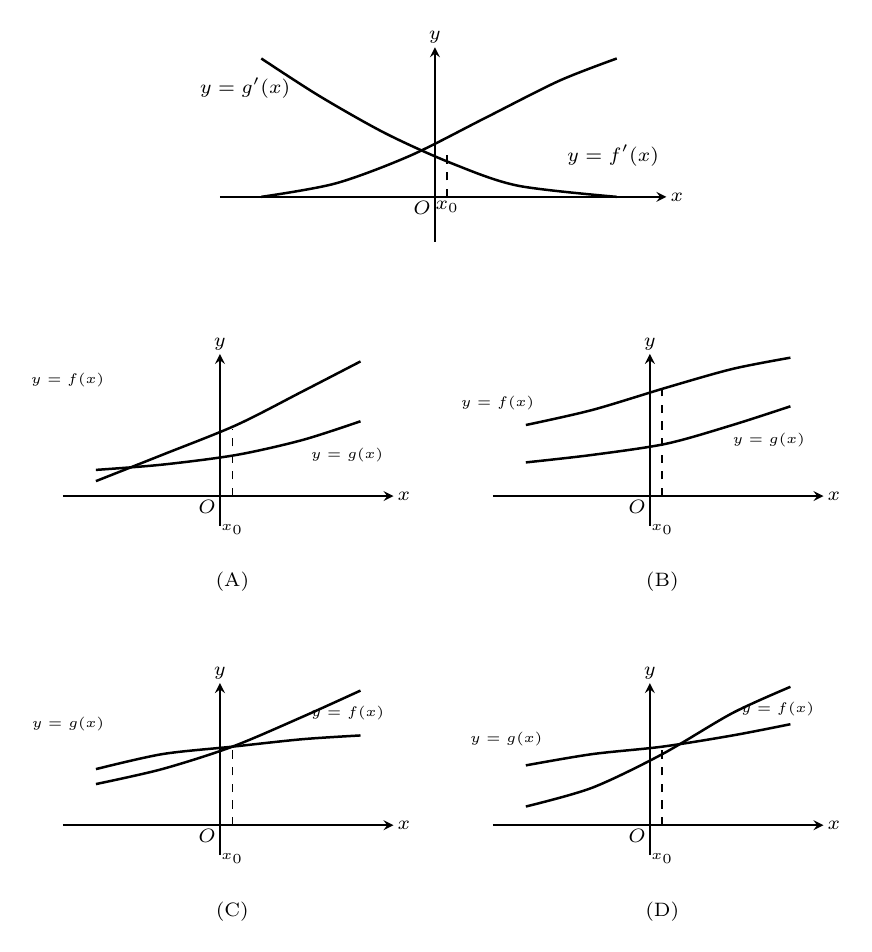
\begin{tikzpicture}[x=1.05cm, y=0.95cm, semithick, font=\scriptsize,
  every node/.style={inner sep=1.2pt}]

  % ---- 题干：导函数图象 ----
  \begin{scope}[shift={(0,0)}]
    \draw[->,>=stealth] (-2.6,0) -- (2.8,0) node[right] {$x$};
    \draw[->,>=stealth] (0,-0.6) -- (0,2.0) node[above] {$y$};
    \node[below left] at (0,0) {$O$};
    \draw[line width=0.9pt, smooth, samples=90]
      plot coordinates {(-2.1,1.85) (-1.4,1.35) (-0.6,0.85) (0.2,0.45) (1.0,0.15) (2.2,0.0)};
    \draw[line width=0.9pt, smooth, samples=90]
      plot coordinates {(-2.1,0.0) (-1.2,0.18) (-0.3,0.55) (0.6,1.05) (1.5,1.55) (2.2,1.85)};
    \draw[dashed] (0.15,0) -- (0.15,0.62);
    \node[below] at (0.15,0) {$x_0$};
    \node[right] at (1.55,0.55) {$y=f'(x)$};
    \node[left] at (-1.70,1.45) {$y=g'(x)$};
  \end{scope}

  % ---- (A) ----
  \begin{scope}[shift={(-2.6,-4.0)}]
    \draw[->,>=stealth] (-1.9,0) -- (2.1,0) node[right] {$x$};
    \draw[->,>=stealth] (0,-0.4) -- (0,1.9) node[above] {$y$};
    \node[below left] at (0,0) {$O$};
    \draw[line width=0.9pt, smooth, samples=90]
      plot coordinates {(-1.5,0.2) (-0.7,0.55) (0.2,0.95) (1.0,1.4) (1.7,1.8)};
    \draw[line width=0.9pt, smooth, samples=90]
      plot coordinates {(-1.5,0.35) (-0.7,0.42) (0.2,0.55) (1.0,0.75) (1.7,1.0)};
    \draw[dashed] (0.15,0) -- (0.15,0.9);
    \node at (0.15,-0.45) {\tiny $x_0$};
    \node[left] at (-1.35,1.55) {\tiny $y=f(x)$};
    \node[right] at (1.05,0.55) {\tiny $y=g(x)$};
    \node at (0.15,-1.15) {(A)};
  \end{scope}

  % ---- (B) ----
  \begin{scope}[shift={(2.6,-4.0)}]
    \draw[->,>=stealth] (-1.9,0) -- (2.1,0) node[right] {$x$};
    \draw[->,>=stealth] (0,-0.4) -- (0,1.9) node[above] {$y$};
    \node[below left] at (0,0) {$O$};
    \draw[line width=0.9pt, smooth, samples=90]
      plot coordinates {(-1.5,0.95) (-0.7,1.15) (0.2,1.45) (1.0,1.7) (1.7,1.85)};
    \draw[line width=0.9pt, smooth, samples=90]
      plot coordinates {(-1.5,0.45) (-0.7,0.55) (0.2,0.7) (1.0,0.95) (1.7,1.2)};
    \draw[dashed] (0.15,0) -- (0.15,1.45);
    \node at (0.15,-0.45) {\tiny $x_0$};
    \node[left] at (-1.35,1.25) {\tiny $y=f(x)$};
    \node[right] at (0.95,0.75) {\tiny $y=g(x)$};
    \node at (0.15,-1.15) {(B)};
  \end{scope}

  % ---- (C) ----
  \begin{scope}[shift={(-2.6,-8.4)}]
    \draw[->,>=stealth] (-1.9,0) -- (2.1,0) node[right] {$x$};
    \draw[->,>=stealth] (0,-0.4) -- (0,1.9) node[above] {$y$};
    \node[below left] at (0,0) {$O$};
    \draw[line width=0.9pt, smooth, samples=90]
      plot coordinates {(-1.5,0.55) (-0.7,0.75) (0.15,1.05) (1.0,1.45) (1.7,1.8)};
    \draw[line width=0.9pt, smooth, samples=90]
      plot coordinates {(-1.5,0.75) (-0.7,0.95) (0.15,1.05) (1.0,1.15) (1.7,1.2)};
    \draw[dashed] (0.15,0) -- (0.15,1.05);
    \node at (0.15,-0.45) {\tiny $x_0$};
    \node[left] at (-1.35,1.35) {\tiny $y=g(x)$};
    \node[right] at (1.05,1.5) {\tiny $y=f(x)$};
    \node at (0.15,-1.15) {(C)};
  \end{scope}

  % ---- (D) ----
  \begin{scope}[shift={(2.6,-8.4)}]
    \draw[->,>=stealth] (-1.9,0) -- (2.1,0) node[right] {$x$};
    \draw[->,>=stealth] (0,-0.4) -- (0,1.9) node[above] {$y$};
    \node[below left] at (0,0) {$O$};
    \draw[line width=0.9pt, smooth, samples=90]
      plot coordinates {(-1.5,0.25) (-0.7,0.5) (0.15,0.95) (1.0,1.5) (1.7,1.85)};
    \draw[line width=0.9pt, smooth, samples=90]
      plot coordinates {(-1.5,0.8) (-0.7,0.95) (0.15,1.05) (1.0,1.2) (1.7,1.35)};
    \draw[dashed] (0.15,0) -- (0.15,1.05);
    \node at (0.15,-0.45) {\tiny $x_0$};
    \node[left] at (-1.25,1.15) {\tiny $y=g(x)$};
    \node[right] at (1.05,1.55) {\tiny $y=f(x)$};
    \node at (0.15,-1.15) {(D)};
  \end{scope}
\end{tikzpicture}
\end{center}
\nopagebreak[4]
\Needspace{4\baselineskip}
\textbf{解析}

在 $x_0$ 处两导函数图象相交，且 $f'$ 递减、$g'$ 递增，故 $f'-g'$ 在 $x_0$ 由正变负，$f-g$ 在 $x_0$ 取极大值，同时两曲线在 $x_0$ 处切线平行。四组图中只有 (C) 满足：$f$ 位于 $g$ 下方且在 $x_0$ 处二者相切。

\gkanswer{答案：C。}

\end{answer}
\begin{answer}
\gksolhead{13}{}

\textbf{题目}：

若 $(x-2)^5=a_5x^5+a_4x^4+a_3x^3+a_2x^2+a_1x+a_0$，则 $a_1+a_2+a_3+a_4+a_5=$\gkblank{}。（用数字作答）

\Needspace{4\baselineskip}
\textbf{解析}

\Needspace{5\baselineskip}
令 $x=1$：

\nopagebreak[4]
\[a_0+a_1+\cdots+a_5=(-1)^5=-1.\]

\Needspace{5\baselineskip}
又 $a_0=(-2)^5=-32$，故

\nopagebreak[4]
\[a_1+a_2+a_3+a_4+a_5=-1+32=31.\]

\gkanswer{答案：$31$。}

\end{answer}
\begin{answer}
\gksolhead{14}{}

\textbf{题目}：

若直线 $3x+4y+m=0$ 与圆 $\begin{cases}x=1+\cos\theta,\\ y=-2+\sin\theta,\end{cases}$（$\theta$ 为参数）没有公共点，则实数 $m$ 的取值范围是\gkblank{}。

\Needspace{4\baselineskip}
\textbf{解析}

\Needspace{5\baselineskip}
圆的参数方程化为 $(x-1)^2+(y+2)^2=1$，圆心 $(1,-2)$，半径 $1$。直线与圆无公共点等价于

\nopagebreak[4]
\[\frac{|3-8+m|}5>1\iff |m-5|>5,\]

解得 $m<0$ 或 $m>10$。

\gkanswer{答案：$(-\infty,0)\cup(10,+\infty)$。}

\end{answer}
\begin{answer}
\gksolhead{15}{}

\textbf{题目}：

若三棱锥的三个侧面两两垂直，且侧棱长均为 $\sqrt3$，则其外接球的表面积是\gkblank{}。

\Needspace{4\baselineskip}
\textbf{解析}

\Needspace{5\baselineskip}
三条侧棱两两垂直且长度均为 $\sqrt3$，可补成以它们为棱的长方体，三棱锥的外接球即长方体的外接球：

\nopagebreak[4]
\[2R=\sqrt{3+3+3}=3,\qquad R=\frac32,\qquad S=4\pi R^2=9\pi.\]

\gkanswer{答案：$9\pi$。}

\end{answer}
\begin{answer}
\gksolhead{16}{}

\textbf{题目}：

设 $P$ 是一个数集，且至少含有两个数，若对任意 $a$、$b\in P$，都有 $a+b$、$a-b$、$ab$、$\dfrac ab\in P$（除数 $b\neq0$），则称 $P$ 是一个数域。例如有理数集 $\mathbf Q$ 是数域；数集 $F=\{a+b\sqrt2\mid a,b\in\mathbf Q\}$ 也是数域。有下列命题：① 整数集是数域；② 若有理数集 $\mathbf Q\subseteq M$，则数集 $M$ 必为数域；③ 数域必为无限集；④ 存在无穷多个数域。其中正确的命题的序号是\gkblank{}。（把你认为正确的命题的序号填填上）

\Needspace{4\baselineskip}
\textbf{解析}

① 整数集中 $1$、$2$ 均在，但 $\dfrac12\notin\mathbf Z$，假；

② 取 $M=\mathbf Q\cup\{\sqrt2\}$，则 $\sqrt2+\sqrt2=2\sqrt2\notin M$，假；

③ 数域含 $1$，故含全部整数与 $\dfrac1n$（$n\in\mathbf N^*$），必为无限集，真；

④ 对每个无平方因子的正整数 $p$，$\{a+b\sqrt p\mid a,b\in\mathbf Q\}$ 都是数域且互不相同，真。

故正确的是 ③④。

\gkanswer{答案：③④。}

\end{answer}
\begin{answer}
\gksolhead{17}{}

\textbf{题目}：

已知向量 $\boldsymbol m=(\sin A,\cos A)$，$\boldsymbol n=(\sqrt3,-1)$，$\boldsymbol m\cdot\boldsymbol n=1$，且 $A$ 为锐角。

（1）求角 $A$ 的大小；

（2）求函数 $f(x)=\cos 2x+4\cos A\sin x$（$x\in\mathbf R$）的值域。

\Needspace{4\baselineskip}
\textbf{解析}

\Needspace{5\baselineskip}
（1）$\boldsymbol m\cdot\boldsymbol n=\sqrt3\sin A-\cos A=1$，即

\nopagebreak[4]
\[2\sin\left(A-\frac{\pi}6\right)=1.\]

由 $A$ 为锐角得 $A-\dfrac{\pi}6\in\left(-\dfrac{\pi}6,\dfrac{\pi}3\right)$，故 $A-\dfrac{\pi}6=\dfrac{\pi}6$，$A=\dfrac{\pi}3$。

\Needspace{5\baselineskip}
（2）由（1）$\cos A=\dfrac12$，故

\nopagebreak[4]
\[f(x)=\cos2x+2\sin x=1-2\sin^2x+2\sin x=-2\left(\sin x-\frac12\right)^2+\frac32.\]

当 $\sin x=\dfrac12$ 时取最大值 $\dfrac32$，当 $\sin x=-1$ 时取最小值 $-3$，值域为 $\left[-3,\dfrac32\right]$。

\gkanswer{答案：（1）$A=\dfrac{\pi}3$；（2）值域 $\left[-3,\dfrac32\right]$。}

\end{answer}
\begin{answer}
\gksolhead{18}{}

\textbf{题目}：

如图，在四棱锥 $P-ABCD$ 中，侧面 $PAD\perp$ 底面 $ABCD$，侧棱 $PA=PD=\sqrt2$，底面 $ABCD$ 为直角梯形，其中 $BC\parallel AD$，$AB\perp AD$，$AD=2AB=2BC=2$，$O$ 为 $AD$ 中点。

（1）求证：$PO\perp$ 平面 $ABCD$；

（2）求异面直线 $PD$ 与 $CD$ 所成角的大小；

（3）线段 $AD$ 上是否存在点 $Q$，使得它到平面 $PCD$ 的距离为 $\dfrac{\sqrt3}{2}$？若存在，求出 $\dfrac{AQ}{QD}$ 的值；若不存在，请说明理由。
\nopagebreak[4]
\begin{center}% 2008 年福建卷理科第 18 题：四棱锥 P-ABCD，侧面 PAD⊥底面 ABCD，PA=PD=√2，
%   底面为直角梯形，BC∥AD，AB⊥AD，AD=2AB=2BC=2，O 为 AD 中点。
% 来源 PDF：gaokaomath-src/普通高考/2008/2008福建理.pdf
% SHA-256：516e8ac8e113868afa9bc4af4724c3b43f22a1f7fecc830a7f3400b8d973d452
% 原页：2008福建理.pdf 第 1 页（A3 三栏）第 3 栏，书页码 441。
% 重绘依据：与文科卷第 19 题同一幅图（同一几何体）：A 左、D 右、O 在 AD 上、B 左下、C 下中、
%   P 在 O 上方；P—A、P—B、P—C、P—D、A—B、B—C、C—D 实线，A—D（含 O）与 P—O 虚线。
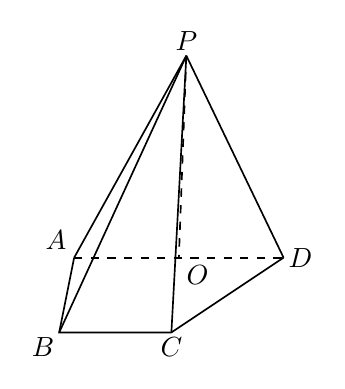
\begin{tikzpicture}[scale=0.95, semithick, every node/.style={inner sep=1.5pt}]
  \coordinate (P) at (1.70,4.00);
  \coordinate (A) at (0.20,1.30);
  \coordinate (D) at (3.00,1.30);
  \coordinate (O) at (1.60,1.30);
  \coordinate (B) at (0.00,0.30);
  \coordinate (C) at (1.50,0.30);

  \draw (P) -- (A);
  \draw (P) -- (B);
  \draw (P) -- (C);
  \draw (P) -- (D);
  \draw (A) -- (B) -- (C) -- (D);
  \draw[dashed] (A) -- (D);
  \draw[dashed] (P) -- (O);

  \node[above] at (P) {$P$};
  \node[above left=1pt] at (A) {$A$};
  \node[right] at (D) {$D$};
  \node[below right=1pt] at (O) {$O$};
  \node[below left] at (B) {$B$};
  \node[below] at (C) {$C$};
\end{tikzpicture}
\end{center}
\nopagebreak[4]
\Needspace{4\baselineskip}
\textbf{解析}

（1）由 $PA=PD$ 且 $O$ 为 $AD$ 中点得 $PO\perp AD$；又平面 $PAD\perp$ 平面 $ABCD$，交线为 $AD$，$PO\subset$ 平面 $PAD$，故 $PO\perp$ 平面 $ABCD$。

\Needspace{5\baselineskip}
（2）以 $A$ 为原点，$AD$、$AB$、平行于 $OP$ 的直线为 $x$、$y$、$z$ 轴，则

\nopagebreak[4]
\[A(0,0,0),\quad B(0,1,0),\quad C(1,1,0),\quad D(2,0,0),\quad P(1,0,1).\]

\Needspace{5\baselineskip}
于是

\nopagebreak[4]
\[\overrightarrow{PD}=(1,0,-1),\qquad \overrightarrow{CD}=(1,-1,0),\]

\nopagebreak[4]
\[\cos\theta=\frac{|\overrightarrow{PD}\cdot\overrightarrow{CD}|}{|\overrightarrow{PD}||\overrightarrow{CD}|}=\frac1{\sqrt2\cdot\sqrt2}=\frac12,\]

故异面直线 $PD$ 与 $CD$ 所成角为 $60^\circ$。

\Needspace{5\baselineskip}
（3）$\overrightarrow{PC}=(0,1,-1)$，$\overrightarrow{PD}=(1,0,-1)$，平面 $PCD$ 的法向量

\nopagebreak[4]
\[\boldsymbol n=\overrightarrow{PC}\times\overrightarrow{PD}=(-1,-1,-1),\]

\Needspace{5\baselineskip}
平面方程为 $x+y+z=2$。设 $Q(t,0,0)$（$0\leqslant t\leqslant2$），则

\nopagebreak[4]
\[d=\frac{|t-2|}{\sqrt3}=\frac{\sqrt3}2\iff |t-2|=\frac32,\]

\Needspace{5\baselineskip}
得 $t=\dfrac12$（$t=\dfrac72>2$ 舍）。故 $AQ=\dfrac12$，$QD=\dfrac32$，

\nopagebreak[4]
\[\frac{AQ}{QD}=\frac13.\]

\gkanswer{答案：（1）证明见解析；（2）$60^\circ$；（3）存在，$\dfrac{AQ}{QD}=\dfrac13$。}

\end{answer}
\begin{answer}
\gksolhead{19}{}

\textbf{题目}：

已知函数 $f(x)=\dfrac13x^3+x^2-2$。

（1）设 $\{a_n\}$ 是正数组成的数列，前 $n$ 项和为 $S_n$，其中 $a_1=3$。若点 $(a_n,a_{n+1}^2-2a_{n+1})$（$n\in\mathbf N^*$）在函数 $y=f'(x)$ 的图象上，求证：点 $(n,S_n)$ 也在 $y=f'(x)$ 的图象上；

（2）求函数 $f(x)$ 在区间 $(a-1,a)$ 内的极值。

\Needspace{4\baselineskip}
\textbf{解析}

\Needspace{5\baselineskip}
（1）$f'(x)=x^2+2x$。由题意

\nopagebreak[4]
\[a_{n+1}^2-2a_{n+1}=a_n^2+2a_n\iff (a_{n+1}-a_n)(a_{n+1}+a_n)=2(a_n+a_{n+1}).\]

\Needspace{5\baselineskip}
因 $a_n>0$，得 $a_{n+1}-a_n=2$，故 $\{a_n\}$ 是首项 $3$、公差 $2$ 的等差数列，$a_n=2n+1$，于是

\nopagebreak[4]
\[S_n=\frac{n(3+2n+1)}2=n(n+2)=n^2+2n=f'(n),\]

即点 $(n,S_n)$ 在 $y=f'(x)$ 的图象上。

（2）$f'(x)=x(x+2)$，故 $f$ 在 $(-\infty,-2)$、$(0,+\infty)$ 上递增，在 $(-2,0)$ 上递减，$x=-2$ 为极大值点，$f(-2)=-\dfrac83+4-2=-\dfrac23$；$x=0$ 为极小值点，$f(0)=-2$。

区间 $(a-1,a)$ 含 $-2$ 当且仅当 $-2<a<-1$，此时只有极大值 $-\dfrac23$；含 $0$ 当且仅当 $0<a<1$，此时只有极小值 $-2$；其余情形（含 $a=-1$、$0$、$1$ 端点）无极值。

\gkanswer{答案：（1）证明见解析；（2）$-2<a<-1$ 时极大值 $-\dfrac23$；$0<a<1$ 时极小值 $-2$；其余情形无极值。}

\end{answer}
\begin{answer}
\gksolhead{20}{}

\textbf{题目}：

某项考试按科目 $A$、科目 $B$ 依次进行，只有当科目 $A$ 成绩合格时，才可继续参加科目 $B$ 的考试。已知每个科目只允许有一次补考机会，两个科目成绩均合格方可获得证书。现某人参加这项考试，科目 $A$ 每次考试成绩合格的概率均为 $\dfrac23$，科目 $B$ 每次考试成绩合格的概率均为 $\dfrac12$。假设各次考试成绩合格与否均互不影响。

（1）求他不需要补考就可获得证书的概率；

（2）在这项考试过程中，假设他不放弃所有的考试机会，记他参加考试的次数为 $\xi$，求 $\xi$ 的数学期望 $E\xi$。

\Needspace{4\baselineskip}
\textbf{解析}

\Needspace{5\baselineskip}
（1）不需补考即两科首次均合格：

\nopagebreak[4]
\[P=\frac23\times\frac12=\frac13.\]

（2）$\xi$ 可取 $2$、$3$、$4$。

$\xi=2$：$A$ 首次合格且 $B$ 首次合格 $\dfrac23\cdot\dfrac12=\dfrac13$，或 $A$ 两次均不合格 $\dfrac13\cdot\dfrac13=\dfrac19$，合计 $\dfrac49$。

$\xi=3$：$A$ 首次合格而 $B$ 补考 $\dfrac23\cdot\dfrac12=\dfrac13$，或 $A$ 补考合格且 $B$ 首次合格 $\dfrac13\cdot\dfrac23\cdot\dfrac12=\dfrac19$，合计 $\dfrac49$。

$\xi=4$：$A$ 补考合格且 $B$ 补考 $\dfrac13\cdot\dfrac23\cdot\dfrac12=\dfrac19$。

\Needspace{5\baselineskip}
故

\nopagebreak[4]
\[E\xi=2\times\frac49+3\times\frac49+4\times\frac19=\frac83.\]

\gkanswer{答案：（1）$\dfrac13$；（2）$E\xi=\dfrac83$。}

\end{answer}
\begin{answer}
\gksolhead{21}{}

\textbf{题目}：

如图，椭圆 $\dfrac{x^2}{a^2}+\dfrac{y^2}{b^2}=1$（$a>b>0$）的一个焦点是 $F(1,0)$，$O$ 为坐标原点。

（1）已知椭圆短轴的两个三等分点与一个焦点构成正三角形，求椭圆的方程；

（2）设过点 $F$ 的直线 $l$ 交椭圆于 $A$、$B$ 两点。若直线 $l$ 绕点 $F$ 任意转动，恒有 $|OA|^2+|OB|^2<|AB|^2$，求 $a$ 的取值范围。
\nopagebreak[4]
\begin{center}% 2008 年福建卷理科第 21 题：椭圆 x²/a²+y²/b²=1（a>b>0），焦点 F(1,0)，O 为原点；
%   过 F 的直线 l 交椭圆于 A、B。
% 来源 PDF：gaokaomath-src/普通高考/2008/2008福建理.pdf
% SHA-256：516e8ac8e113868afa9bc4af4724c3b43f22a1f7fecc830a7f3400b8d973d452
% 原页：2008福建理.pdf 第 2 页（A3 三栏）第 2 栏，书页码 442。
% 重绘依据：按原页画椭圆与 x/y 轴，F 在 x 轴正半轴上；过 F 的直线 l 与椭圆交于
%   第一象限的 A 与第三象限的 B。取图示椭圆 x 半径 2.6、y 半径 1.75，A、B 取在椭圆上
%   且与 F 共线（A≈(1.99,1.13)、B≈(−0.51,−1.72)），l 在两端各延长一小段。
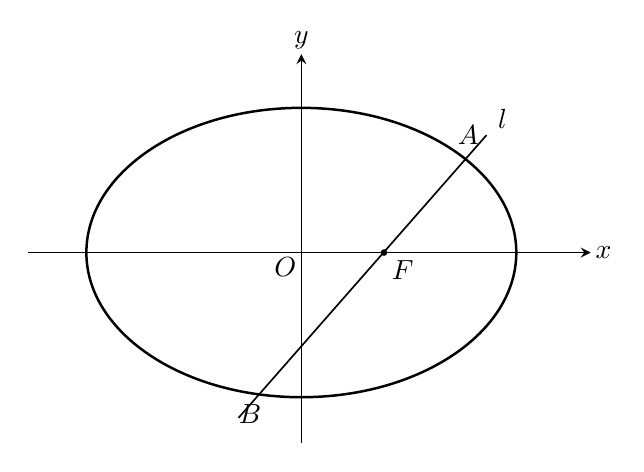
\begin{tikzpicture}[x=1.05cm, y=1.05cm, semithick, every node/.style={inner sep=1.5pt}]
  \draw[->,>=stealth] (-3.3,0) -- (3.5,0) node[right] {$x$};
  \draw[->,>=stealth] (0,-2.3) -- (0,2.4) node[above] {$y$};
  \node[below left] at (0,0) {$O$};

  \draw[line width=0.9pt] (0,0) ellipse [x radius=2.6, y radius=1.75];

  \coordinate (F) at (1,0);
  \coordinate (A) at (1.99,1.13);
  \coordinate (B) at (-0.51,-1.72);

  \draw (-0.76,-2.00) -- (2.24,1.42);
  \node[right] at (2.32,1.62) {$l$};

  \fill (F) circle (1.2pt);
  \node[below right=1pt] at (F) {$F$};
  \node at (2.02,1.42) {$A$};
  \node at (-0.62,-1.95) {$B$};
\end{tikzpicture}
\end{center}
\nopagebreak[4]
\Needspace{4\baselineskip}
\textbf{解析}

\Needspace{5\baselineskip}
（1）短轴的两个三等分点为 $\left(0,\pm\dfrac b3\right)$，与 $F(1,0)$ 构成正三角形，故

\nopagebreak[4]
\[\sqrt{1+\frac{b^2}9}=\frac{2b}3\iff 1+\frac{b^2}9=\frac{4b^2}9\iff b^2=3.\]

\Needspace{5\baselineskip}
又 $c=1$，$a^2=b^2+c^2=4$，椭圆为

\nopagebreak[4]
\[\frac{x^2}4+\frac{y^2}3=1.\]

\Needspace{5\baselineskip}
（2）直线 $l$ 的参数方程取为 $x=1+t\cos\theta$，$y=t\sin\theta$，代入椭圆并记 $b^2=a^2-1$：

\nopagebreak[4]
\[\left(\frac{\cos^2\theta}{a^2}+\frac{\sin^2\theta}{b^2}\right)t^2+\frac{2\cos\theta}{a^2}t+\frac1{a^2}-1=0.\]

\Needspace{5\baselineskip}
记 $A_l=\dfrac{\cos^2\theta}{a^2}+\dfrac{\sin^2\theta}{b^2}$，则 $t_1t_2=\dfrac{1/a^2-1}{A_l}$，$t_1+t_2=-\dfrac{2\cos\theta}{a^2A_l}$，且

\nopagebreak[4]
\[\overrightarrow{OA}\cdot\overrightarrow{OB}=1+t_1t_2-\frac{2\cos^2\theta}{a^2A_l}.\]

\Needspace{5\baselineskip}
题设条件等价于 $\overrightarrow{OA}\cdot\overrightarrow{OB}<0$ 对一切 $\theta$ 成立。取 $\theta=\dfrac{\pi}2$，此时 $A_l=\dfrac1{b^2}$，

\nopagebreak[4]
\[\overrightarrow{OA}\cdot\overrightarrow{OB}=1-\frac{(a^2-1)^2}{a^2}=3-a^2-\frac1{a^2},\]

\Needspace{5\baselineskip}
要求其为负，需 $a^2+\dfrac1{a^2}>3$，即 $a^4-3a^2+1>0$，解得 $a^2>\dfrac{3+\sqrt5}2$，故

\nopagebreak[4]
\[a>\frac{1+\sqrt5}2.\]

（$\theta=\dfrac{\pi}2$ 是最不利方向：其余方向上 $\overrightarrow{OA}\cdot\overrightarrow{OB}$ 更小。）

\gkanswer{答案：（1）$\dfrac{x^2}4+\dfrac{y^2}3=1$；（2）$a>\dfrac{1+\sqrt5}2$。}

\end{answer}
\begin{answer}
\gksolhead{22}{}

\textbf{题目}：

已知函数 $f(x)=\ln(1+x)-x$。

（1）求 $f(x)$ 的单调区间；

（2）记 $f(x)$ 在区间 $[0,\pi]$（$n\in\mathbf N^*$）上的最小值为 $b_n$，令 $a_n=\ln(1+n)-b_n$。

① 如果对一切 $n$，不等式 $\sqrt{a_n}<\sqrt{a_{n+2}}-\dfrac{c}{\sqrt{a_{n+2}}}$ 恒成立，求实数 $c$ 的取值范围；

② 求证：$\dfrac{a_1}{a_2}+\dfrac{a_1a_3}{a_2a_4}+\cdots+\dfrac{a_1a_3\cdots a_{2n-1}}{a_2a_4\cdots a_{2n}}<\sqrt{2a_n+1}-1$。

\Needspace{4\baselineskip}
\textbf{解析}

【源疑点：原页印「在区间 $[0,\pi]$（$n\in\mathbf N^*$）上的最小值为 $b_n$」。区间与 $n$ 无关则 $b_n$ 为常数，与 $a_n=\ln(1+n)-b_n$、$\sqrt{2a_n+1}$ 不能自洽；按 $[0,n]$ 理解则 $a_n=n$，两问均有确定结论。题面照原页转录，作答按 $[0,n]$ 口径。】

（1）$f'(x)=\dfrac1{1+x}-1=-\dfrac x{1+x}$（$x>-1$），故 $f$ 在 $(-1,0)$ 上递增、在 $(0,+\infty)$ 上递减。

\Needspace{5\baselineskip}
（2）$f$ 在 $[0,n]$ 上递减，故 $b_n=f(n)=\ln(1+n)-n$，

\nopagebreak[4]
\[a_n=\ln(1+n)-b_n=n.\]

\Needspace{5\baselineskip}
① 条件即 $\sqrt n<\sqrt{n+2}-\dfrac c{\sqrt{n+2}}$，等价于

\nopagebreak[4]
\[c<(n+2)-\sqrt{n(n+2)}=\frac{2(n+2)}{(n+2)+\sqrt{n(n+2)}}.\]

右端随 $n$ 递减且趋于 $1$（$n=1$ 时为 $3-\sqrt3$），故对一切 $n$ 恒成立当且仅当 $c\leqslant1$。

\Needspace{5\baselineskip}
② 记 $t_k=\dfrac{1\cdot3\cdots(2k-1)}{2\cdot4\cdots2k}$，则

\nopagebreak[4]
\[t_k^2=\prod_{j=1}^k\frac{(2j-1)^2}{4j^2}<\prod_{j=1}^k\frac{2j-1}{2j+1}=\frac1{2k+1},\]

\Needspace{5\baselineskip}
即 $t_k<\dfrac1{\sqrt{2k+1}}$。又

\nopagebreak[4]
\[\sqrt{2k+1}-\sqrt{2k-1}=\frac2{\sqrt{2k+1}+\sqrt{2k-1}}>\frac1{\sqrt{2k+1}}>t_k,\]

\Needspace{5\baselineskip}
逐项求和得

\nopagebreak[4]
\[\sum_{k=1}^n t_k<\sum_{k=1}^n\left(\sqrt{2k+1}-\sqrt{2k-1}\right)=\sqrt{2n+1}-1,\]

即所证不等式成立。

\gkanswer{答案：（1）增区间 $(-1,0)$，减区间 $(0,+\infty)$；（2）① $c\leqslant1$；② 证明见解析。}

\end{answer}